\documentclass{article}
\usepackage{hyperref}
\usepackage[utf8]{inputenc}
\usepackage[margin=12.7mm]{geometry}
\usepackage{helvet}
\usepackage{graphicx}
\usepackage{color}
\usepackage[parfill]{parskip}
\usepackage{titlesec}
\graphicspath{{./images/}}
\titleformat*{\section}{\LARGE\bfseries}
\titleformat*{\subsection}{\Large\bfseries}
\renewcommand{\familydefault}{\sfdefault}
\author{G12}
\title{Documento di sviluppo dell’applicazione}
\date{}
\begin{document}
   \maketitle 
   \tableofcontents
   \clearpage
   \section{Scopo del documento}
   Il presente documento riporta tutte le informazioni necessarie per lo sviluppo di un aspetto dell'applicazione SmartFit. In particolare, presenta tutti gli artefatti necessari per realizzare i servizi di gestione delle funzionalità di un utente non allenatore (da ora semplicemente “utente”) dell’applicazione SmartFit. 
   Purtroppo non abbiamo potuto svolgere questo lavoro per l’utente di tipo allenatore poiché le funzionalità in più per quel tipo di utente riguardavano l’interazione tra più utenti e la creazione, eliminazione e condivisione di file plain text e non. Si è deciso di svolgere quindi il più possibile per quanto riguarda le funzionalità associate a un utente trattandole e sviluppandole in modo molto dettagliato.\\
   Sono state quindi descritte tutte le user stories per l’utente dell’applicazione, comprendendo tutte le funzionalità che erano descritte nel documento di specifiche del progetto nel modo più completo possibile. Partendo da questo, si sono individuate le varie features da implementare. Da queste ultime sono state sviluppate le varie API necessarie, di cui è stata svolta la completa ed esaustiva documentazione. Delle principali API è stata svolta anche una fase di testing con input corretti ed errati per dimostrare il loro funzionamento. Infine, sono stati realizzati front end e back end per poter visualizzare le varie API in opera in una riproduzione del front end fornito nel primo documento dal gruppo G11.
   \section{User stories}
   Una “User Story” è una spiegazione informale e generale di una funzionalità o caratteristica del software che viene descritta dall’utente finale. In pratica serve per dire quali funzionalità servono all’utente, e il motivo per cui gli servono.
   In questo documento le varie User Stories vanno a descrivere le necessità dell’utente nell’applicazione SmartFit.
   Le User Stories non sono scritte in modo formale o con un linguaggio tecnico. Sono bensì in linguaggio naturale, servono solo per rispondere alle domande: “A chi serve qualcosa?”, “Cosa gli serve?”, e, necessariamente, “Perché gli serve?”. Questo processo verrà eseguito per ogni singola    funzionalità che si avrà intenzione di implementare, ovvero tutte quelle associate ad un utente di SmartFit.
   Si riporta ora la tabella con tutte le User Stories legate all’utente dell’applicazione SmartFit.
   \begin{center}
      \begin{tabular}{|c|p{10cm}|c|c|}
         \hline
         \# & Descrizione user story & Requisiti funzionali & Requisiti non funzionali\\
         \hline
         US1 & Come utente, voglio inserire i pasti che assumo, così posso tenerne traccia. Voglio anche avere la possibilità di eliminare l’ultimo pasto inserito nel caso in cui compissi un errore di inserimento. & RF7 &\\
         \hline
         US2 & Come utente, voglio inserire i miei allenamenti così posso tenerne traccia. Voglio anche avere la possibilità di eliminare l’ultima attività inserita nel caso in cui compissi un errore di inserimento. & RF7 & \\
         \hline
         US3 & Come utente, voglio visualizzare i valori nutrizionali di ciò che assumo, in modo da poter gestire la mia dieta in modo efficace & RF6 &\\
         \hline
         US4 & Come utente, voglio visualizzare la mia cronologia dei pasti assunti e attività svolte, così posso tenere traccia dei miei progressi nel tempo & RF6 & \\
         \hline
         US5 & Come utente, voglio visualizzare il mio riepilogo giornaliero sia di dieta che di allenamento così ho una panoramica immediata sul mio andamento giornaliero & RF5 & \\
         \hline
         US6 & Come utente, voglio visualizzare, nel riepilogo giornaliero, il bilancio energetico, e un semplice grafico che mi permetta di mettere a confronto i macro nutrienti che assumo, così posso rendermi conto se sto sbagliando qualcosa nella mia alimentazione & RF5 & \\
         \hline
         US7 & Come utente, voglio visualizzare, nel riepilogo giornaliero, i principali micronutrienti che ho assunto durante la giornata così posso rendermi conto se la mia dieta è bilanciata & RF5 & \\
         \hline
         US8 & Come utente, voglio poter visualizzare le schede personalizzate che mi ha inviato il mio allenatore, così posso averle a portata di mano e poterle utilizzare & RF9 & RNF9\\
         \hline
         US9 & Come utente, voglio poter visualizzare delle informazioni sul mio allenatore, così posso verificare la sua identità & RF10 & \\
         \hline
         US10 & Come utente, voglio poter inserire le attività fisiche svolte non solo manualmente ma anche da un dispositivo esterno al sistema & RF8 & \\
         \hline
      \end{tabular}
   \end{center}
   \section{Features}
   \begin{center}
      \begin{tabular}{|c|c|p{10cm}|}
         \hline
         User Story & Feature Index & Feature\\
         \hline 
         US1 & F1 & Delle caselle di testo per inserire le informazioni e un pulsante che permette di aggiungere un nuovo pasto\\
         \hline
         US1 & F2 & Per permettere l’eliminazione di un pasto inserito sarà presente un pulsante a fianco ad ogni voce del riepilogo giornaliero, descritto successivamente\\
         \hline 
         US2 & F3 & Delle caselle di testo per inserire le informazioni e un pulsante che permette di aggiungere una nuova attività\\
         \hline
         US2 & F4 & Per permettere l’eliminazione di un’attività inserita sarà presente un pulsante a fianco ad ogni voce del riepilogo giornaliero, descritto successivamente\\
         \hline 
         US3 & F5 & Utilizzo di un database esterno per recuperare le informazioni nutrizionali sugli alimenti consumati\\
         \hline
         US4 & F6 & Mostra le liste di pasti assunti e attività svolte. Le cronologie di dieta e allenamento saranno salvate su due file JSON locali\\
         \hline
         US5 & F7 & Mostra la lista giornaliera di pasti assunti e attività svolte nella giornata corrente\\
         \hline 
         US6 & F8 & Nella schermata di riepilogo giornaliero (pagina principale dell’app), verrà mostrato un conteggio per il bilancio energetico\\
         \hline
         US6 & F9 & Nella schermata di riepilogo giornaliero verrà mostrato un grafico, con delle progress bar, che metterà a confronto le quantità di macronutrienti assunti\\
         \hline
         US7 & F10 & Nella schermata di riepilogo giornaliero, verrà mostrata una lista di micronutrienti con i rispettivi quantitativi assunti durante la giornata\\
         \hline
         US8 & F11 & In una schermata, verranno mostrate le due schede personalizzate, di allenamento e dieta, le quali verranno importate tramite file plain text locali\\
         \hline 
         US9 & F12 & Mostra le generalità dell’allenatore in una schermata adibita, recuperate da un file JSON locale\\
         \hline
         US10 & F13 & La API di inserimento di un’attività fisica prende come input un file JSON contenente le informazioni sull’allenamento dell’utente in modo da essere molto generale e poter essere adattata in caso la si voglia collegare all’API esterna per un dispositivo smart\\
         \hline         
      \end{tabular}
   \end{center}
   \newpage
   \section{User Flow}
   In questa sezione del documento si riportano gli “User Flows” per il ruolo dell’utente. L’immagine che segue descrive lo user flow relativo alle varie funzioni trattate in questa fase di sviluppo. Sarà anche presente una breve legenda che descrive i simboli utilizzati.\\
   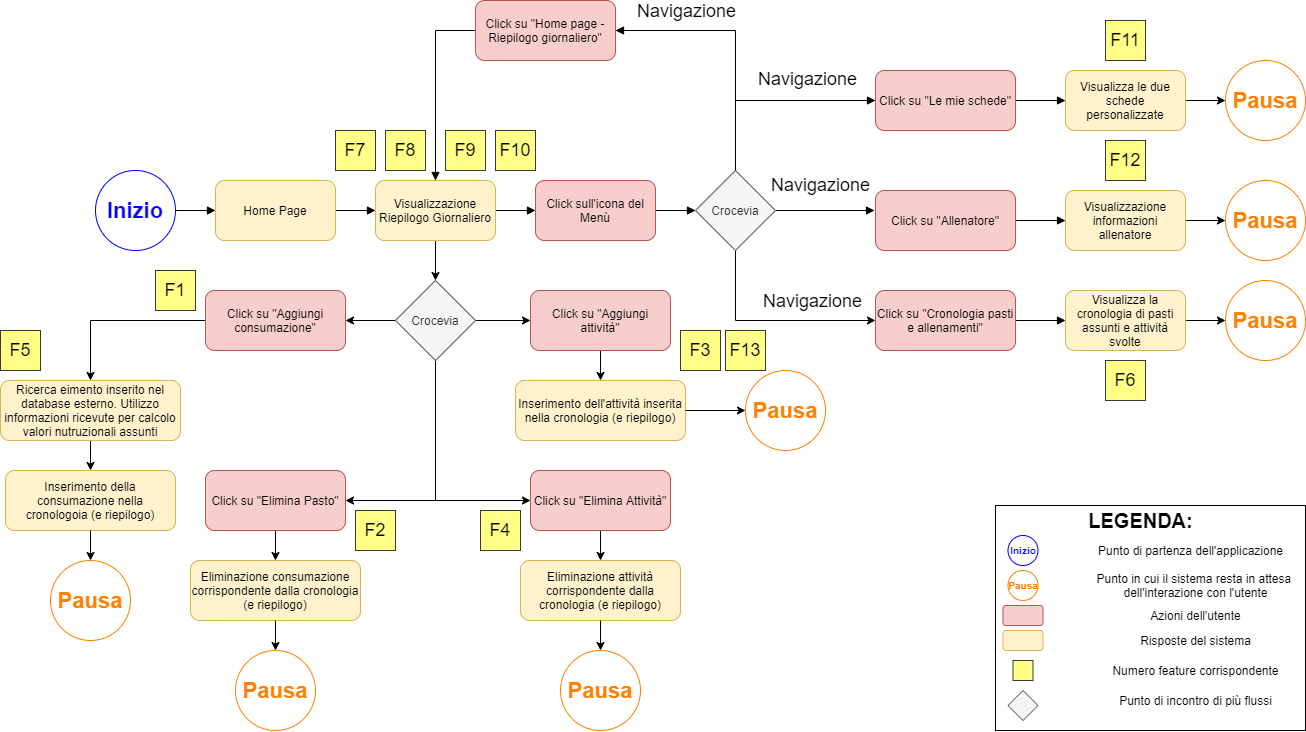
\includegraphics[scale=0.4]{User Flow.drawio.png}
   \section{Application Implementation and Documentation}
   Nelle sezioni precedenti del presente documento, abbiamo identificato le varie features individuate partendo dalle varie User Stories. Queste features individuate devono essere ora implementate. L’applicazione è stata sviluppata con HTML e CSS per quanto riguarda il front end e JavaScript per il back end e per le API. Si è inoltre fatto uso di MongoDB per la gestione dei dati dei valori nutrizionali degli alimenti.
   \subsection{Project Structure}
   La struttura del codice sorgente del progetto è presentata nella figura sottostante. Il progetto è composto delle cartelle:
   \begin{itemize}
      \item \textbf{api} per la gestione delle api locali e in cui è contenuto anche lo script per il testing, nella sottocartella \textbf{test}
      \item \textbf{cronologie} in cui sono presenti le cronologie di alimentazione e di allenamento dell’utente
      \item \textbf{data} in cui sono presenti le schede personalizzate dell’utente e le informazioni sull’allenatore
      \item \textbf{static} in cui è presente tutto il codice che riguarda la User Interface, quindi front end e back end con HTML, CSS e JavaScript.
   \end{itemize}
   \begin{center}
      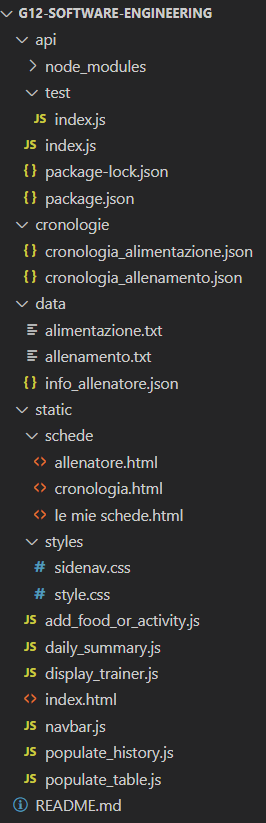
\includegraphics[scale=0.5]{struttura.png}
   \end{center}
   \subsection{Project Dependencies}
   Per la realizzazione dell’applicazione vari moduli sono stati utilizzati e aggiunti al Package.json. Si riporta lo screenshot della sezione nel package.json:\\
   \begin{center}
      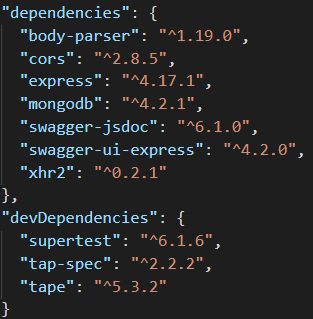
\includegraphics[scale=0.5]{dipendenze.png}
   \end{center}
   \subsection{Project Data or DB}
   Per la gestione dei dati utili all’applicazione abbiamo definito una struttura dati “Food” con MongoDB in cui abbiamo inserito alcuni alimenti/pasti per poter provare le APIs sviluppate.
   Gli alimenti inseriti sono: Mela, Pera, Banana, Kiwi, Lattuga, Cipolla, Pollo, Manzo, Risotto, Pasta al pomodoro, ecc.\\
   Per ogni elemento presente nel database abbiamo inserito dei valori nutrizionali di esempio, su 100 grammi di consumazione. I macronutrienti sono espressi in grammi, mentre i micronutrienti sono espressi in milligrammi.\\
   I dati salvati per ogni elemento sono: nome, energia, grassi, carboidrati, proteine, fibre, ferro, iodio, magnesio.
   La decisione su quali macro e micronutrienti dovessimo inserire è stata presa insieme al gruppo G11, dato che nelle specifiche del progetto non era stato dichiarato tale dato.
   Si riporta un esempio di elemento presente nel database:\\
   \begin{center}
      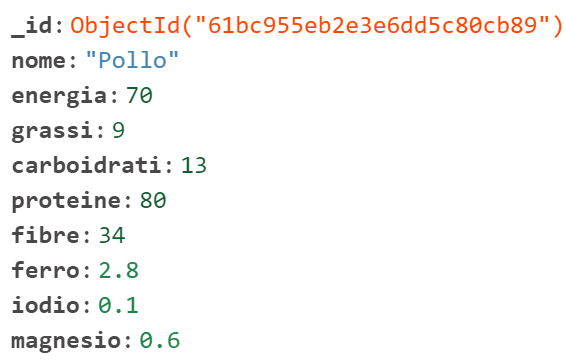
\includegraphics[scale=0.5]{pollo.png}
   \end{center}
   La stringa di connessione al database verrà fornita in una sezione successiva.
   \subsection{Project APIs}
   Seguono la lista e una breve descrizione delle API che sono state sviluppate per questo progetto. La descrizione completa per ogni API può essere trovata nella sezione che riguarda la documentazione. Per quanto riguarda il codice, si può trovare il link alla repository di GitHub in una sezione successiva.
   \newline
   \textbf{GET APIs}\\  
   Segue la lista di API di tipo GET che sono state sviluppate.
   \begin{itemize}
      \item Dati allenatore: recupera le informazioni riguardanti l’allenatore, in formato JSON.
      \item Cronologia alimentazione: recupera la cronologia della dieta dell’utente, in formato JSON.
      \item Cronologia allenamento: recupera la cronologia dell’allenamento dell’utente, in formato JSON.
      \item Riepilogo alimentazione: recupera il riepilogo giornaliero della cronologia della dieta dell’utente (consumazioni nella giornata corrente), in formato JSON.
      \item Riepilogo allenamento: recupera il riepilogo giornaliero  dalla cronologia dell’allenamento dell’utente (attività svolte nella giornata corrente), in formato JSON.
   \end{itemize}
   \textbf{POST APIs}\\
   Segue la lista di API di tipo POST che sono state sviluppate.
   \begin{itemize}
      \item Cronologia allenamento: inserisce l’attività fornita tramite formato JSON nella cronologia dell’allenamento dell’utente.
      \item Cronologia alimentazione: inserisce la consumazione fornita tramite parametro nella cronologia della dieta dell’utente.
   \end{itemize}
   \textbf{DELETE APIs}\\
   Segue la lista di API di tipo DELETE che sono state sviluppate.
   \begin{itemize}
      \item Cronologia allenamento: elimina l’attività fornita tramite parametro dalla cronologia della dieta dell’utente.
      \item Cronologia alimentazione: elimina la consumazione fornita tramite parametro dalla cronologia della dieta dell’utente.
   \end{itemize}
   \textbf{Utility APIs}\\
   Segue la lista di API che sono state sviluppate e che vengono utilizzate o come supporto di altre API (la prima) o per recuperare dei dati per poi mostrarli all’utente come richiesto nella lista delle features.
   \begin{itemize}
      \item GET:
         \begin{itemize}
            \item Valori nutrizionali: recupera le informazioni nutrizionali di un alimento passato come parametro contattando il database remoto.
            \item Calorie assunte: restituisce l’assunzione energetica giornaliera da parte dell’utente, in kcal.
            \item Calorie bruciate: restituisce l’energia bruciata dall’utente nella giornata corrente, in kcal.
            \item Assunzione giornaliera: restituisce la quantità assunta nella giornata corrente del valore nutrizionale passato come parametro. La quantità è espressa in grammi per i macronutrienti e in milligrammi per i micronutrienti.
         \end{itemize}
   \end{itemize}
   \section{API documentation}
   Le API locali fornite dall’applicazione SmartFit elencate nella sezione precedente sono state interamente documentate utilizzando il modulo NodeJS chiamato Swagger UI Express. In particolare, le API sono state annotate utilizzando JSDoc: uno strumento la cui funzione è di generare una documentazione partendo da commenti inseriti nel codice sorgente. Swagger UI invece è stato utilizzato per creare un endpoint in cui si può visualizzare una pagina web con l’intera documentazione.
   L’endpoint si trova all’indirizzo: \textit{localhost:5000/api-docs}\\
   Di seguito viene riportata l’immagine della pagina web relativa alla documentazione.\\
   \\
   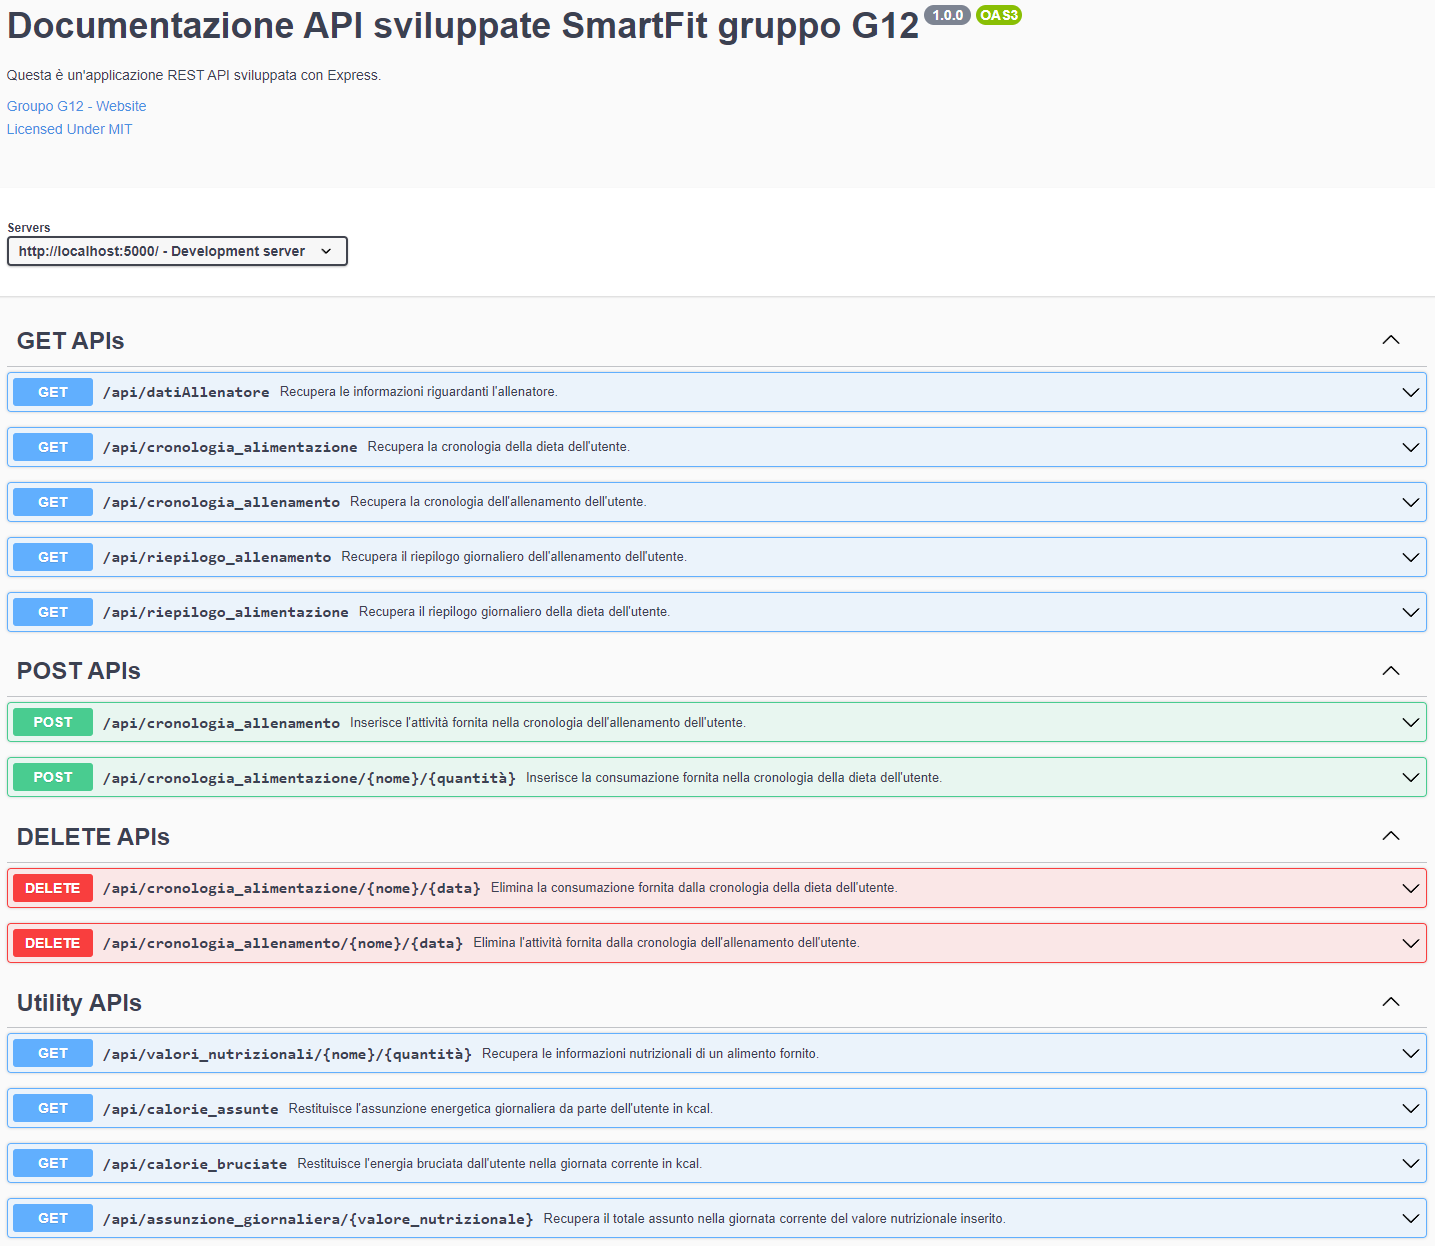
\includegraphics[scale=0.5]{documentazione.png}\\
   \\
   Si descrive ora l’utilizzo delle API più importanti con l’aiuto della documentazione. Per non creare un documento enorme, non ci si dilungherà molto nella spiegazione del funzionamento, essendoci il codice disponibile su GitHub e molti dettagli sono già scritti negli screenshot della documentazione che verranno riportati.
   Le GET sono tutte abbastanza simili, si porta l’esempio della cronologia allenamento:\\
   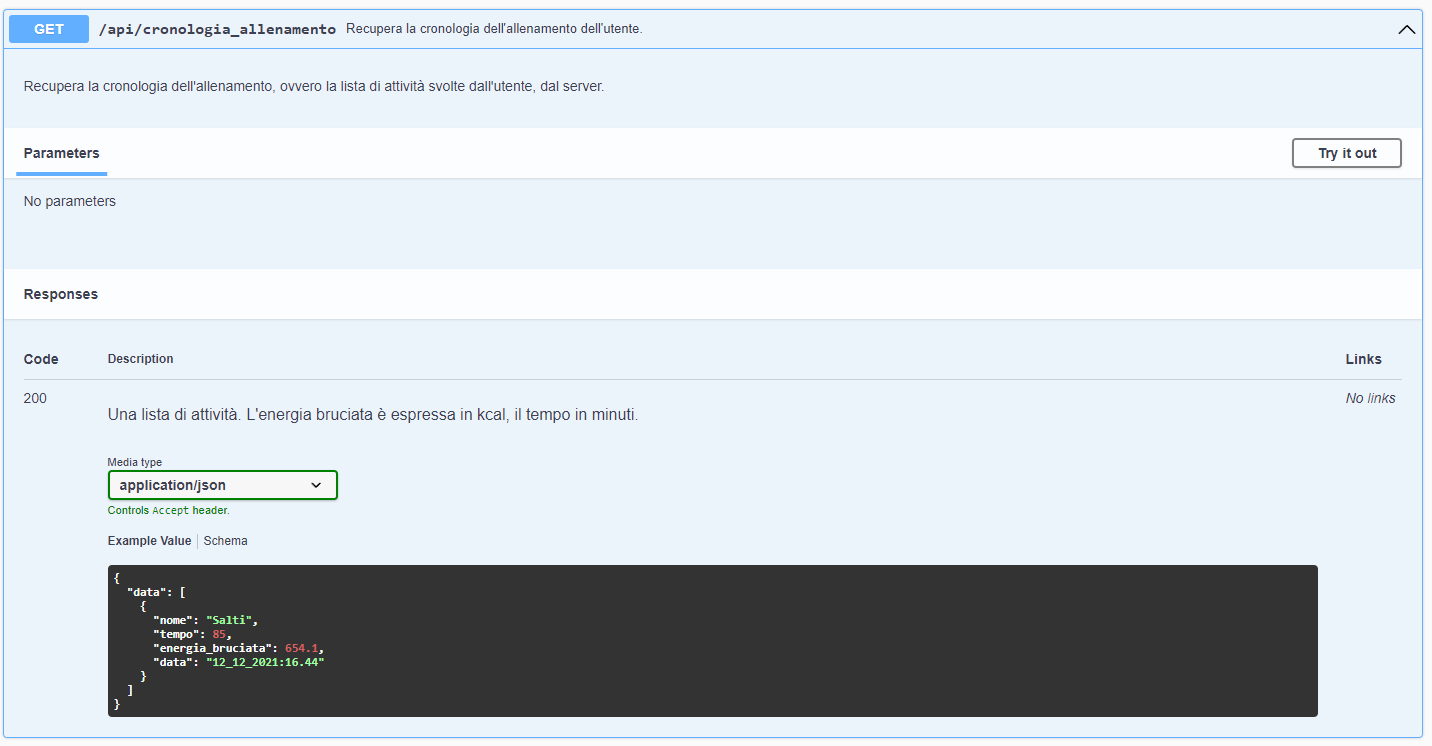
\includegraphics[scale=0.5]{doc get cronologia_allenamento.png}\\
   Quando viene chiamata, l’API ritorna tutta la cronologia dell’allenamento dell’utente. In pratica va a prendere il JSON contenente tale cronologia e lo invia:\\
   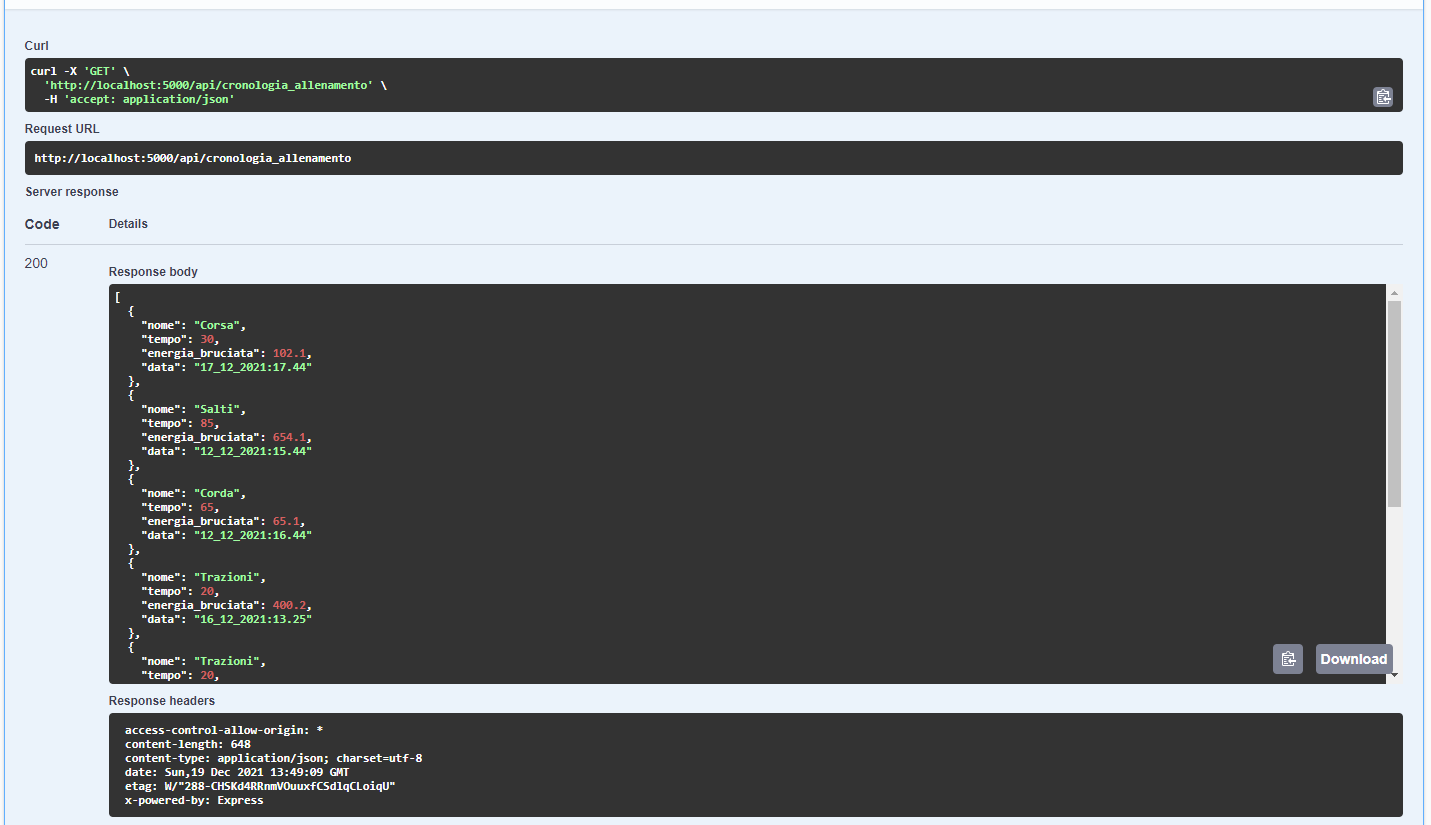
\includegraphics[scale=0.5]{risposta get cronologia_allenamento.png}\\
   \\
   Le API GET “dati allenatore” e “cronologia alimentazione” sono praticamente uguali, solo che ritornano file JSON diversi, ovviamente. Per quanto riguarda le API GET “riepilogo alimentazione” e “riepilogo allenamento”, il funzionamento è molto simile solo che svolgono una fase di filtraggio del JSON della cronologia, ovvero costruiscono un JSON a partire da quello della cronologia inserendo solo gli elementi la cui data corrisponde con quella della giornata corrente, per poi inviarlo come risposta.


   Le due POST API sono leggermente diverse, anche se la funzione è simile.
   La API POST “cronologia alimentazione” prende come parametri (path parameters) il nome e la quantità di un determinato alimento consumato dall’utente:\\
   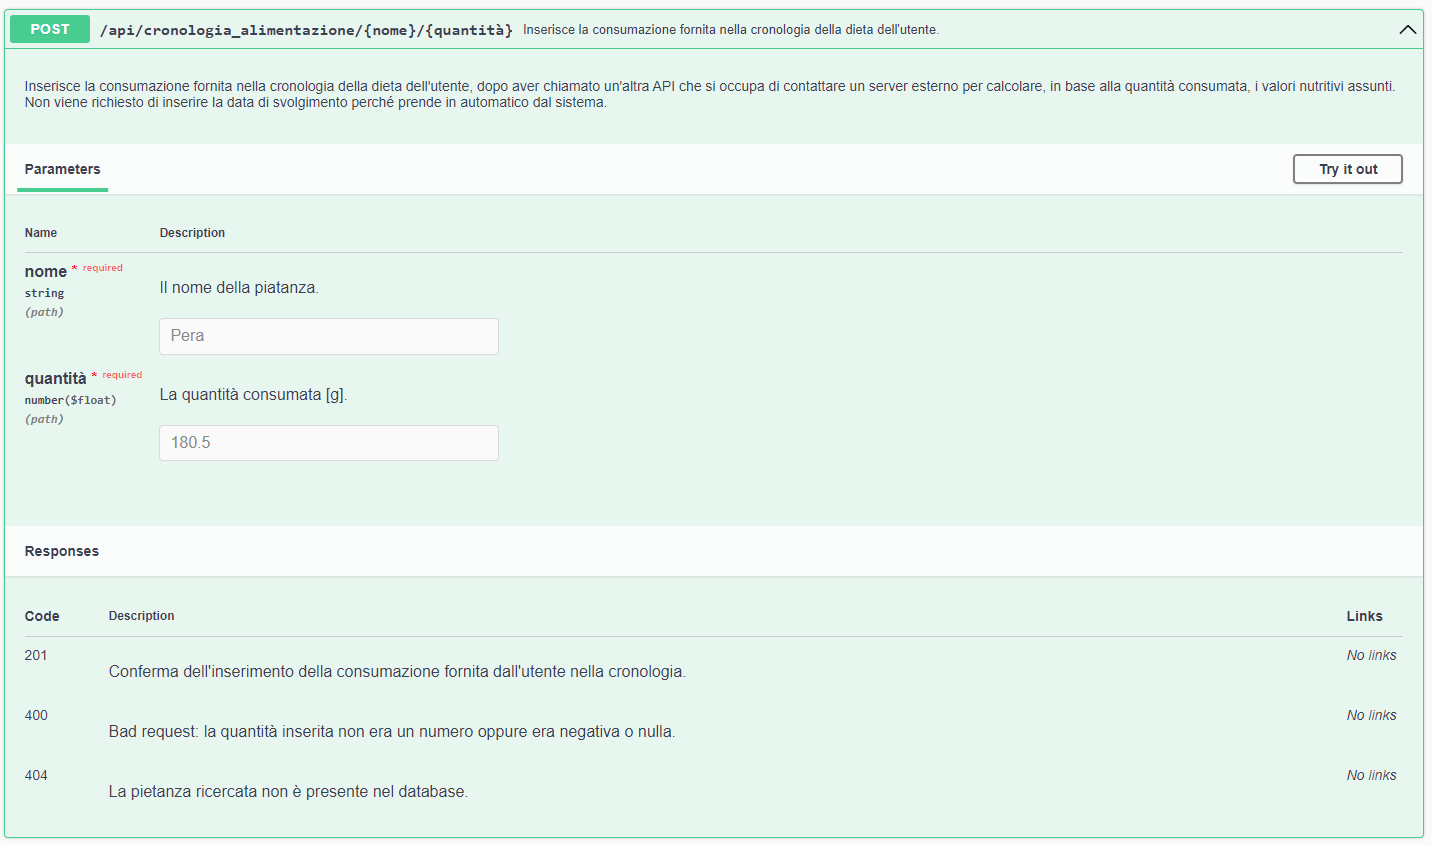
\includegraphics[scale=0.5]{doc post cronologia_alimentazione.png}\\
   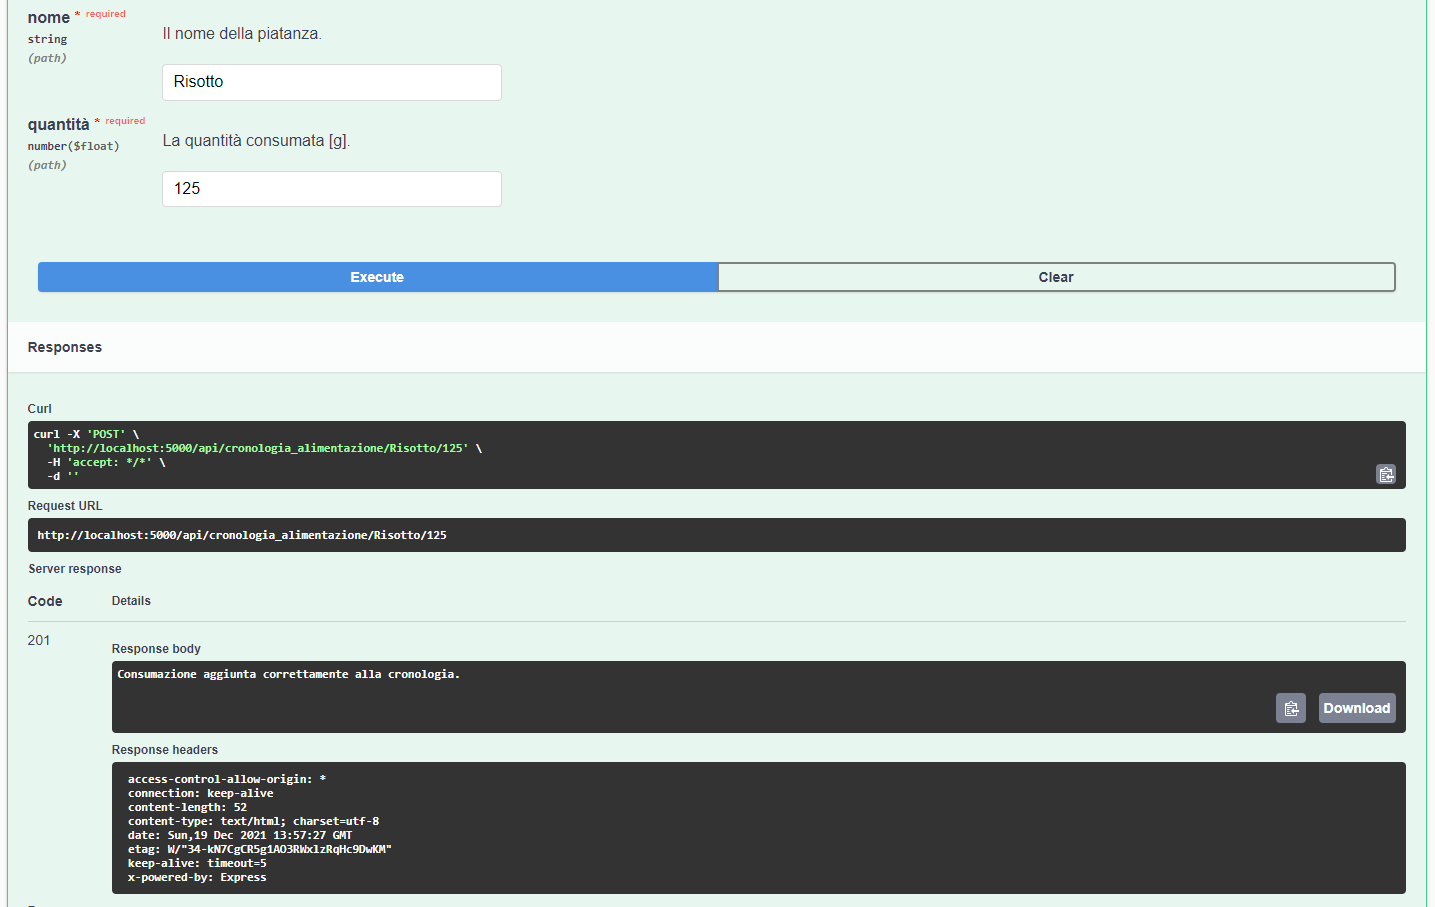
\includegraphics[scale=0.5]{risposta post cronologia_alimentazione.png}\\


   Per quanto riguarda la API POST “cronologia allenamento” l’unica cosa che cambia è che l’input non viene passato come path parameter bensì come body della richiesta, in ofrmato JSONF:\\
   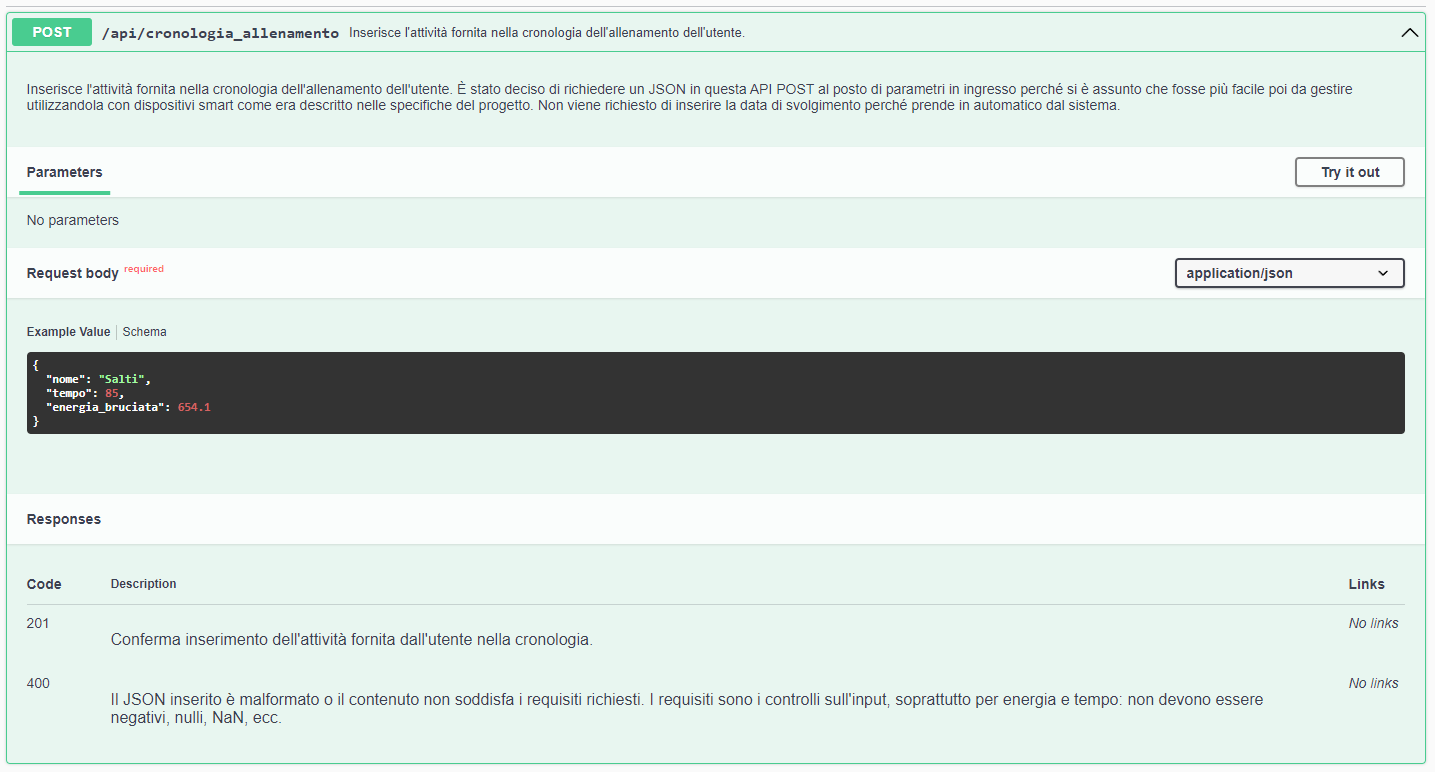
\includegraphics[scale=0.5]{doc post cronologia_allenamento.png}\\
   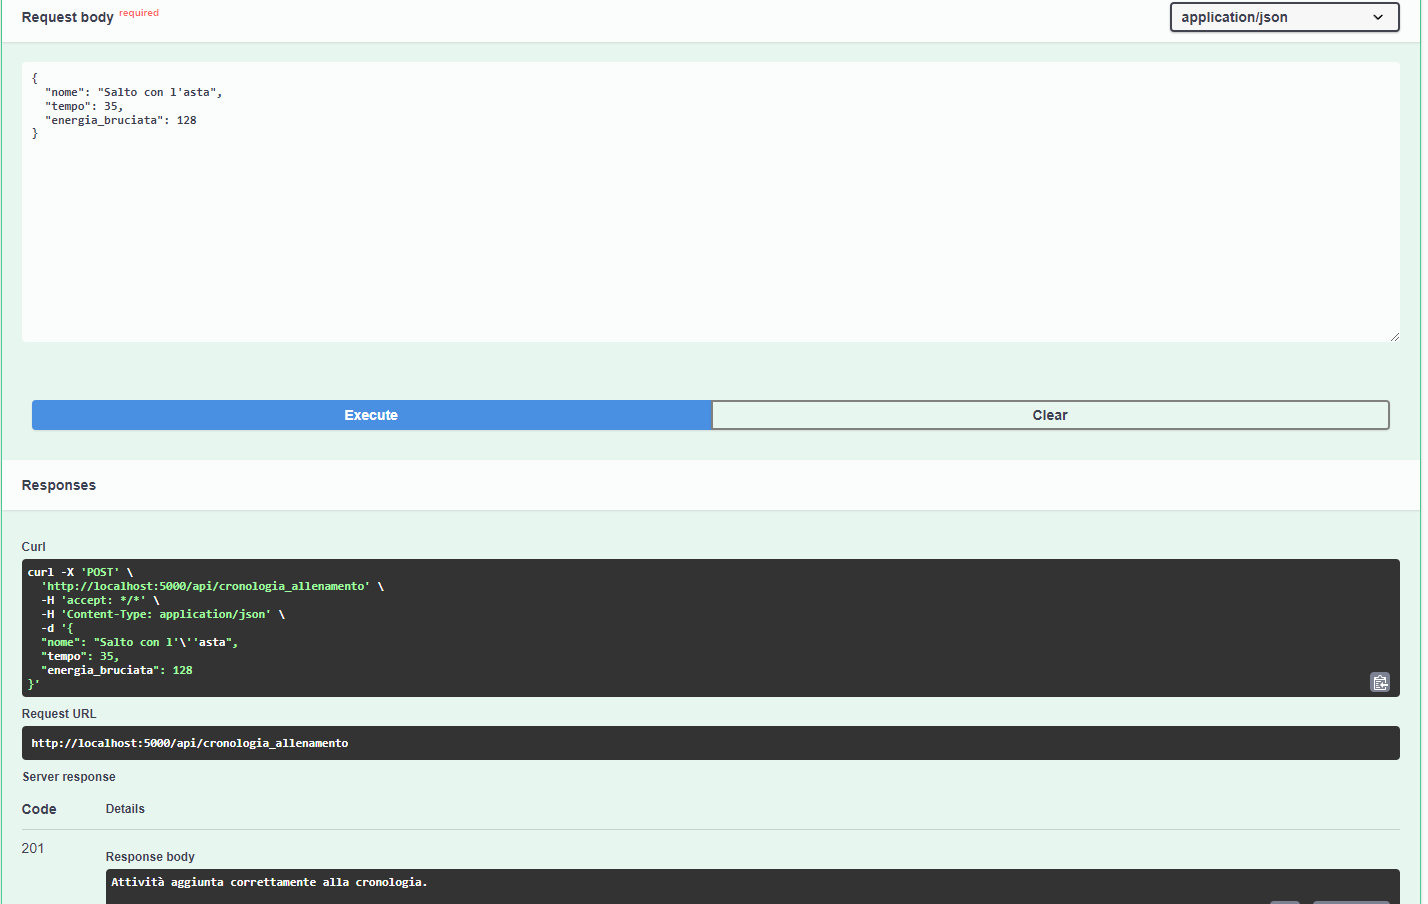
\includegraphics[scale=0.5]{risposta post cronologia_allenamento.png}\\
   \\
   \\
   Si riporta ora una delle due API DELETE, dato che sono molto simili.\\
   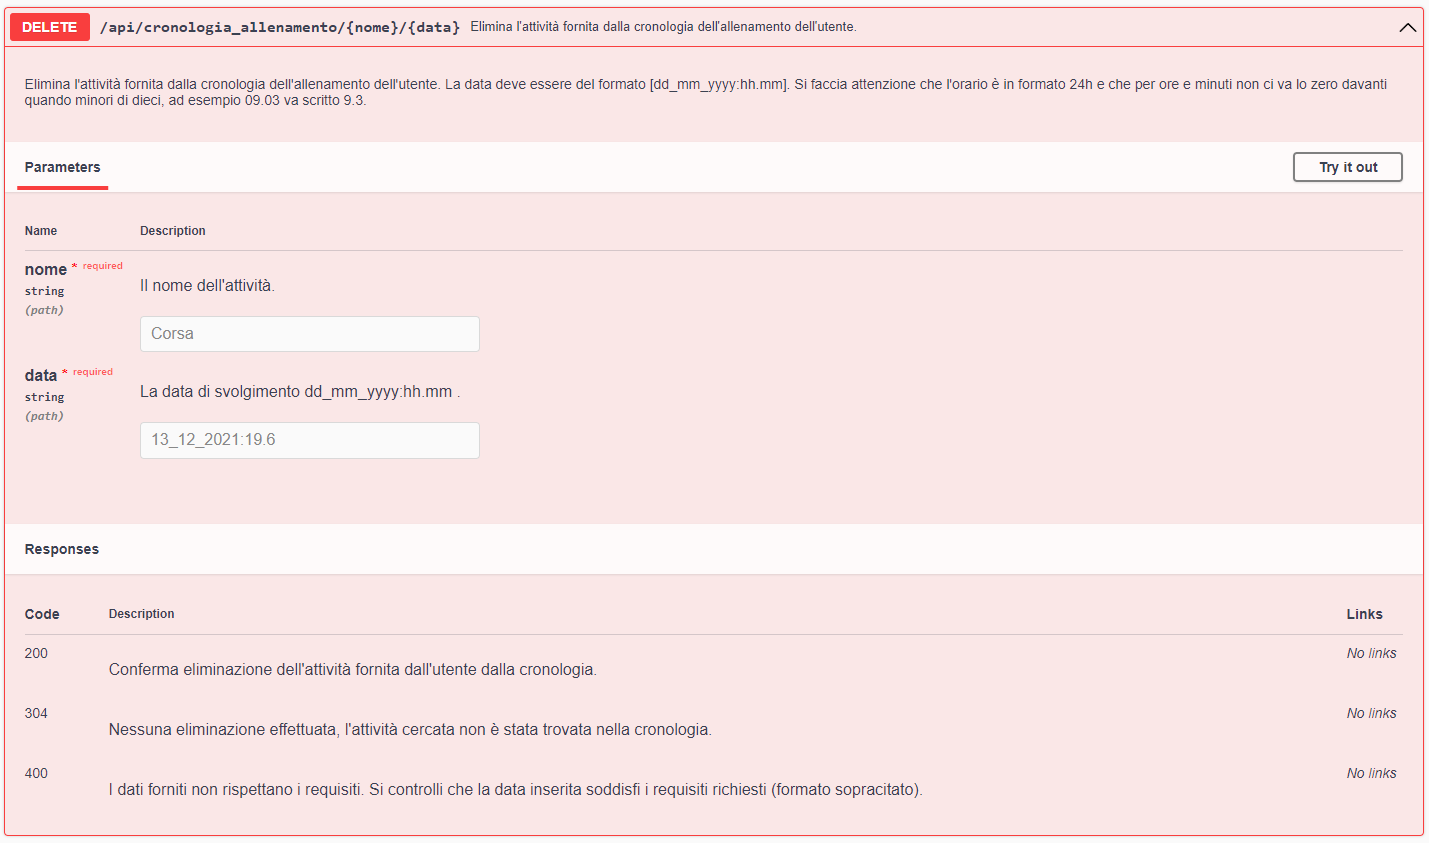
\includegraphics[scale=0.5]{doc delete cronologia_allenamento.png}\\
   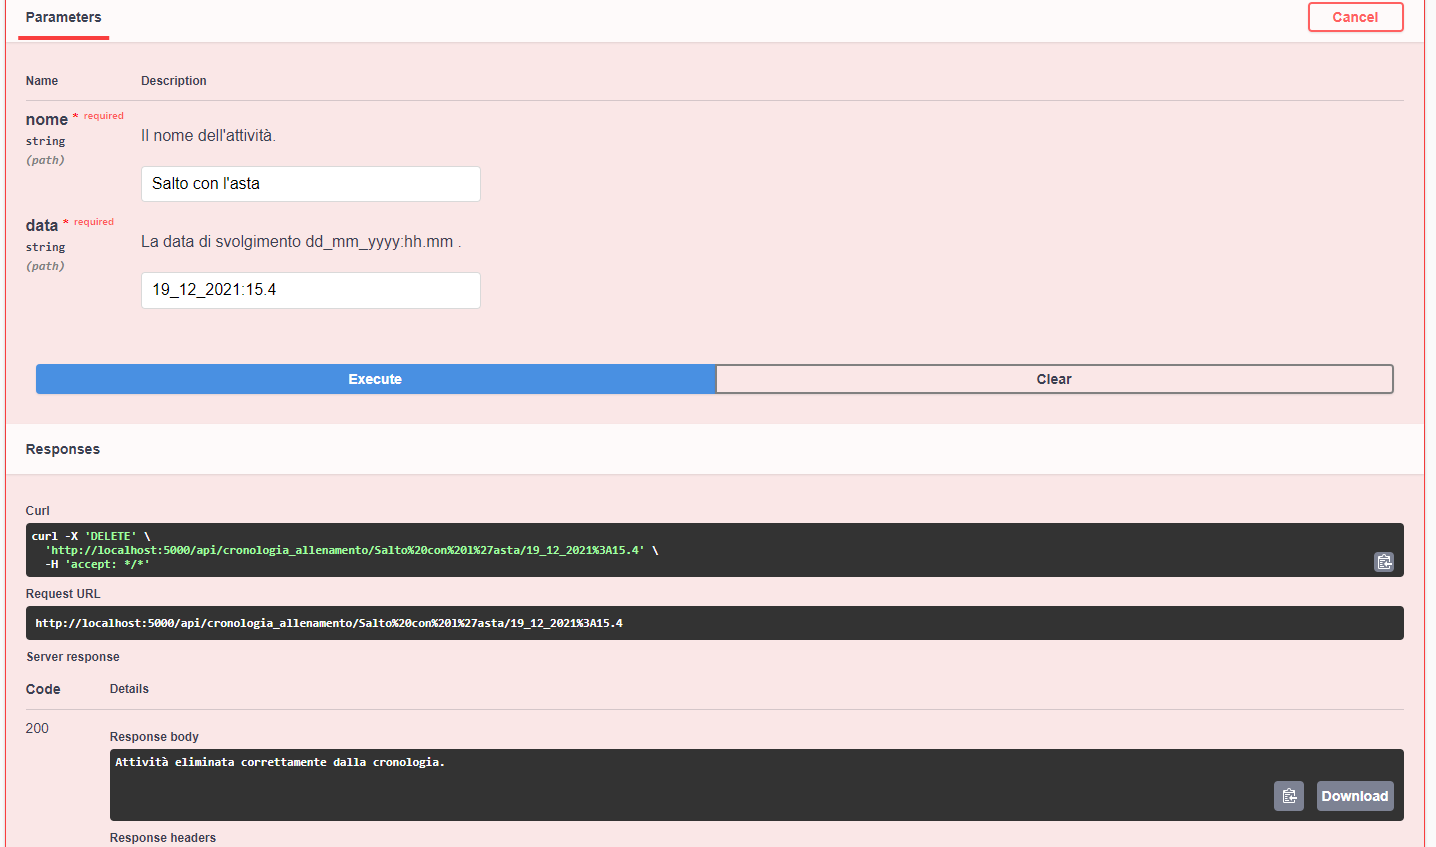
\includegraphics[scale=0.5]{risposta delete cronologia_allenamento.png}
   \\
   \\
   Le Utility API GET “calorie assunte” e “calorie bruciate” sono abbastanza banali, si riporta solo lo screenshot della documentazione di una delle due:\\
   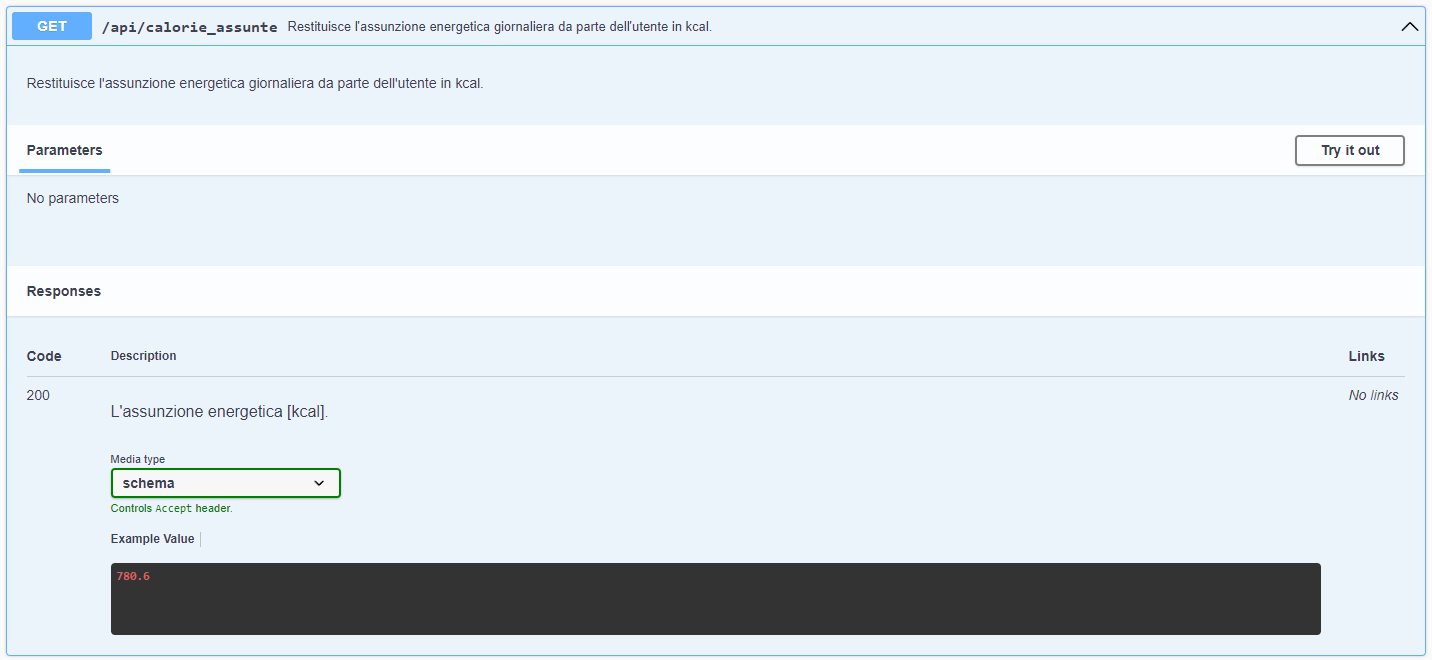
\includegraphics[scale=0.5]{doc get calorie_assunte.png}\\
   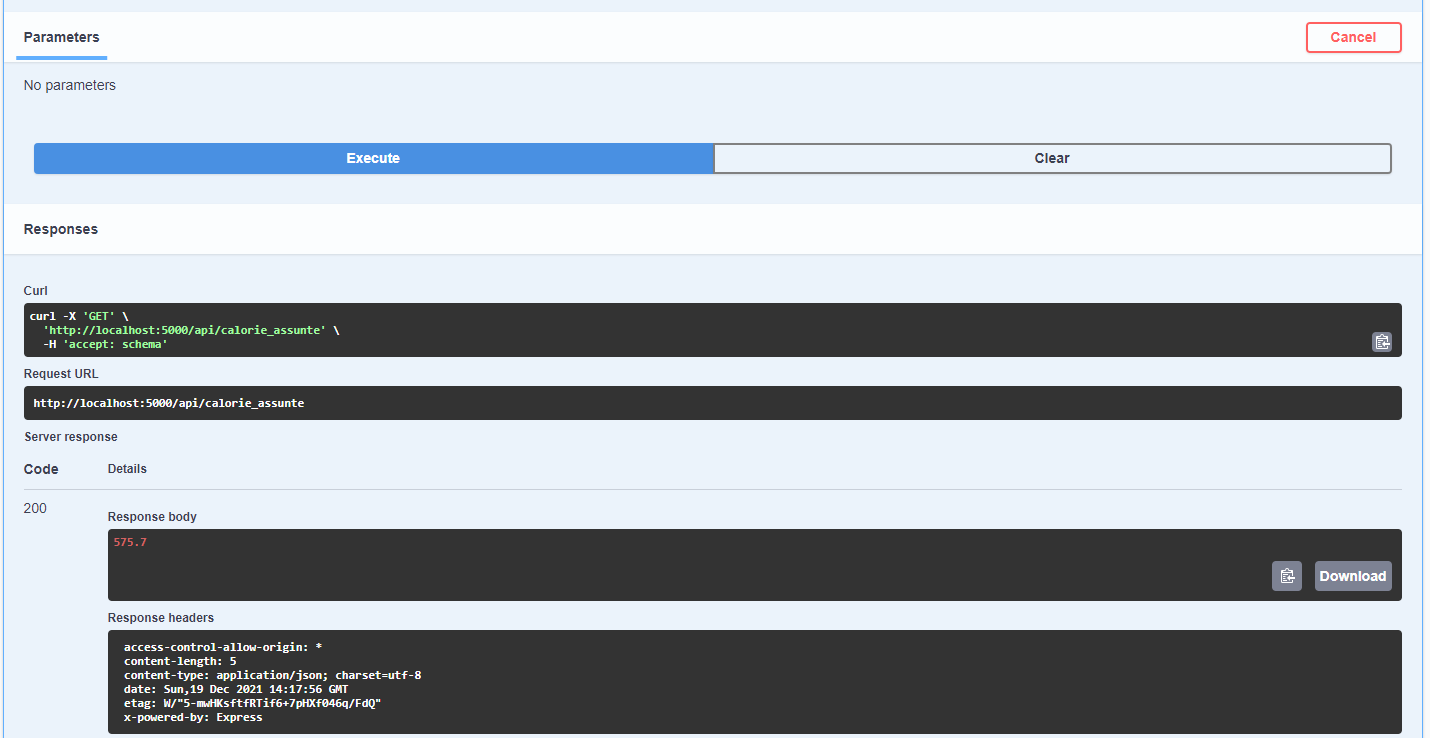
\includegraphics[scale=0.5]{risposta get calorie_assunte.png}
   \\
   \\
   La Utility API GET "valori\_nutrizionali" è quella che si occupa della connessione con il database MongoDB eseguendo una findOne() con il nome dell'alimento che l'utente passa come parametro di ingresso (path parameter).\\
   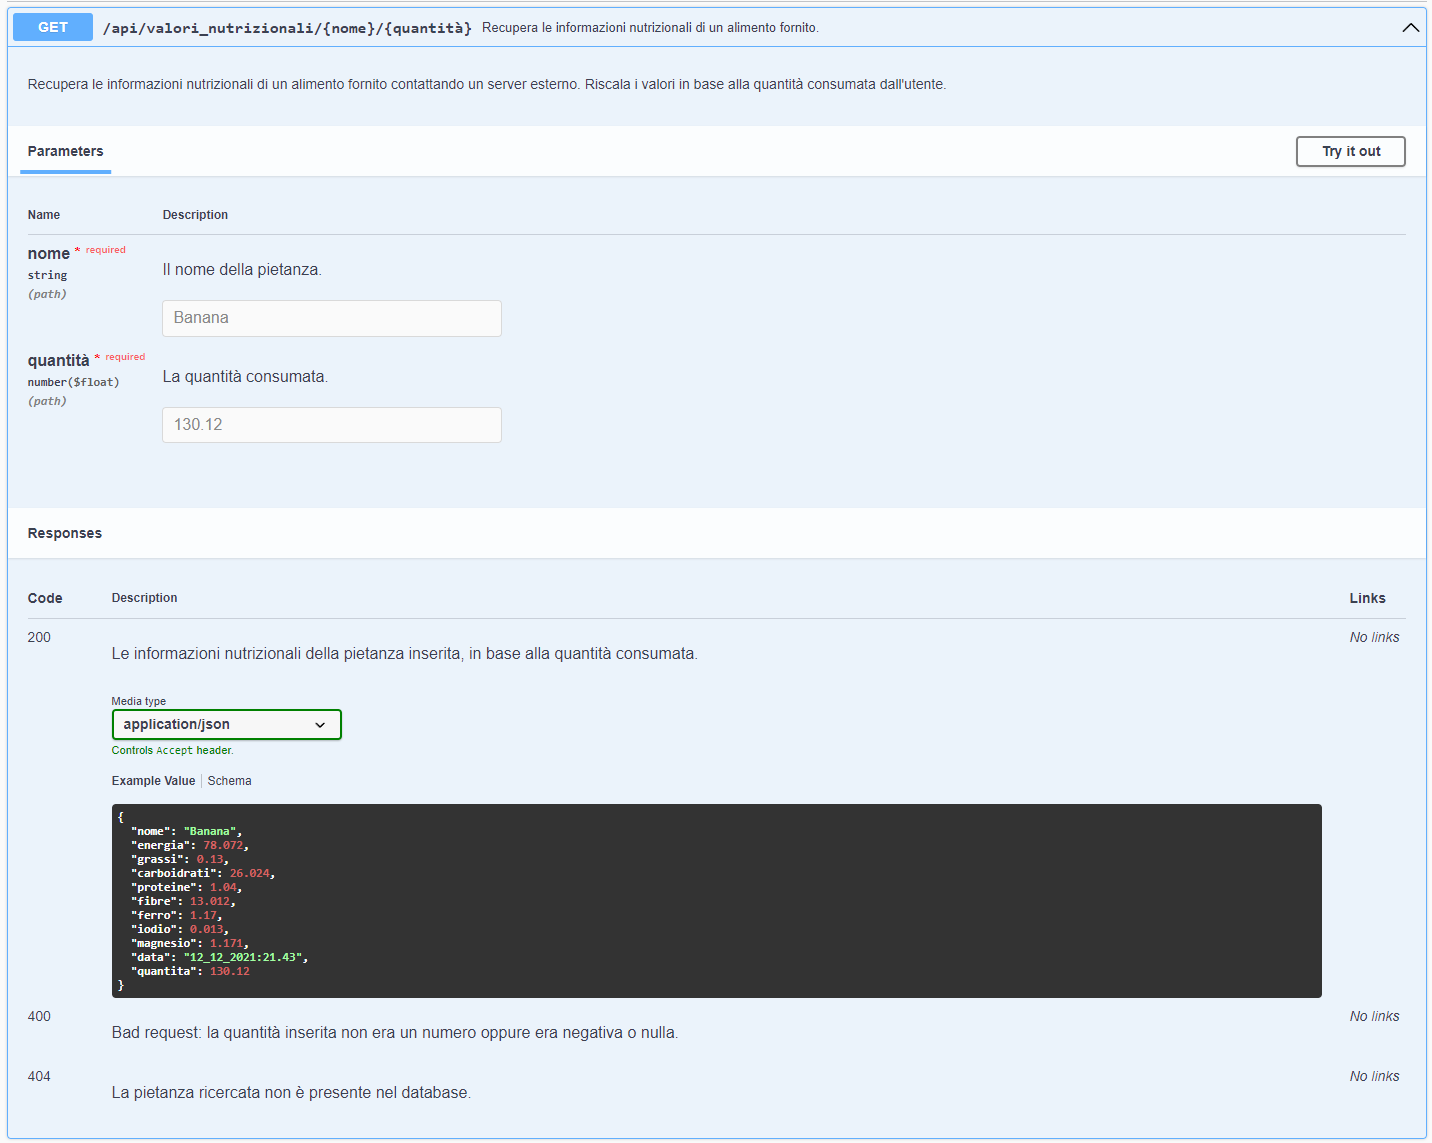
\includegraphics[scale=0.5]{doc get valori_nutrizionali.png}\\
   \\
   Infine, la Utility GET API "assunzione giornaliera":\\
   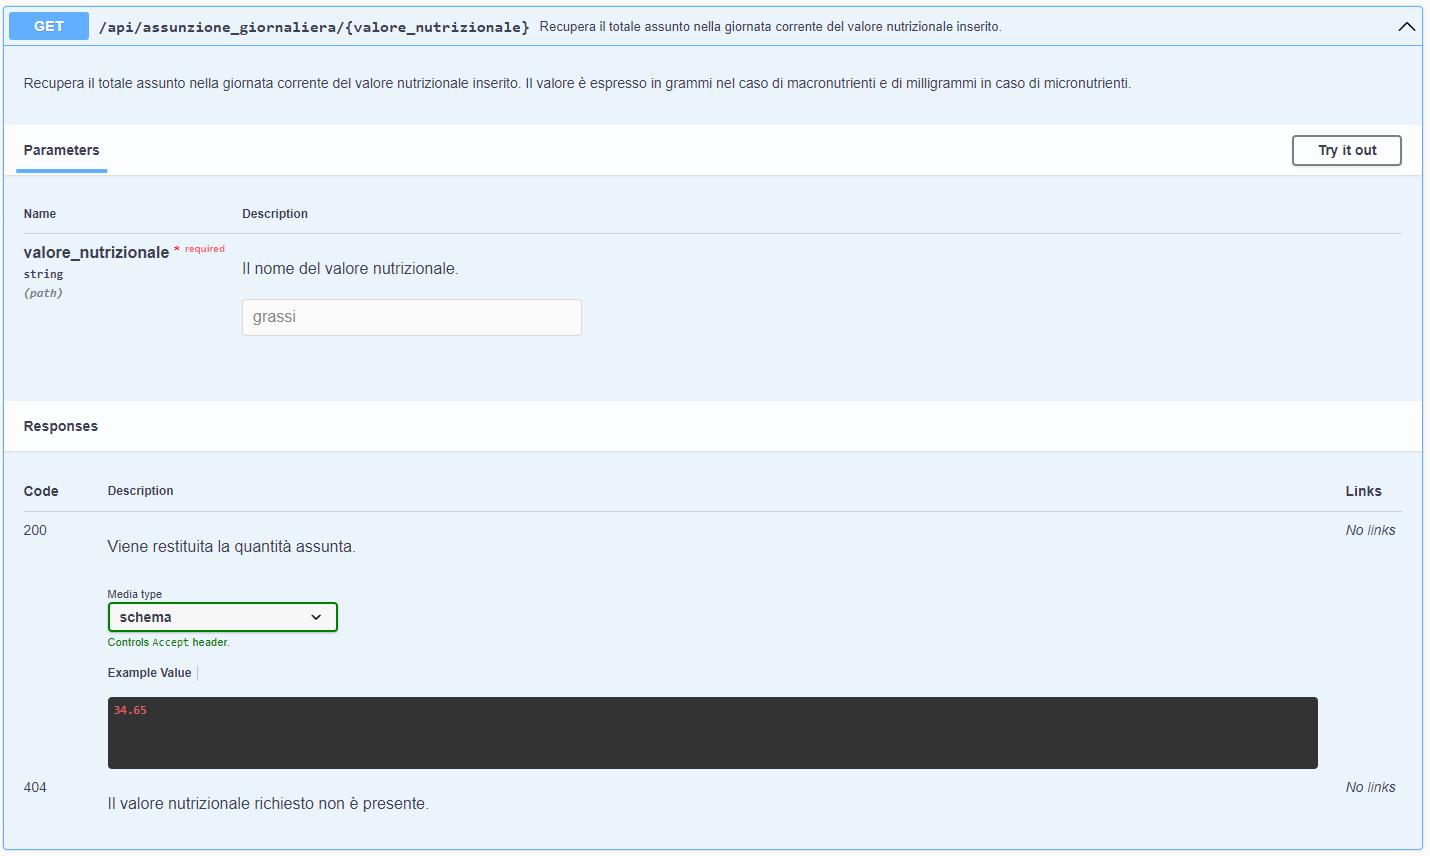
\includegraphics[scale=0.5]{doc get assunzione_giornaliera.png}\\
   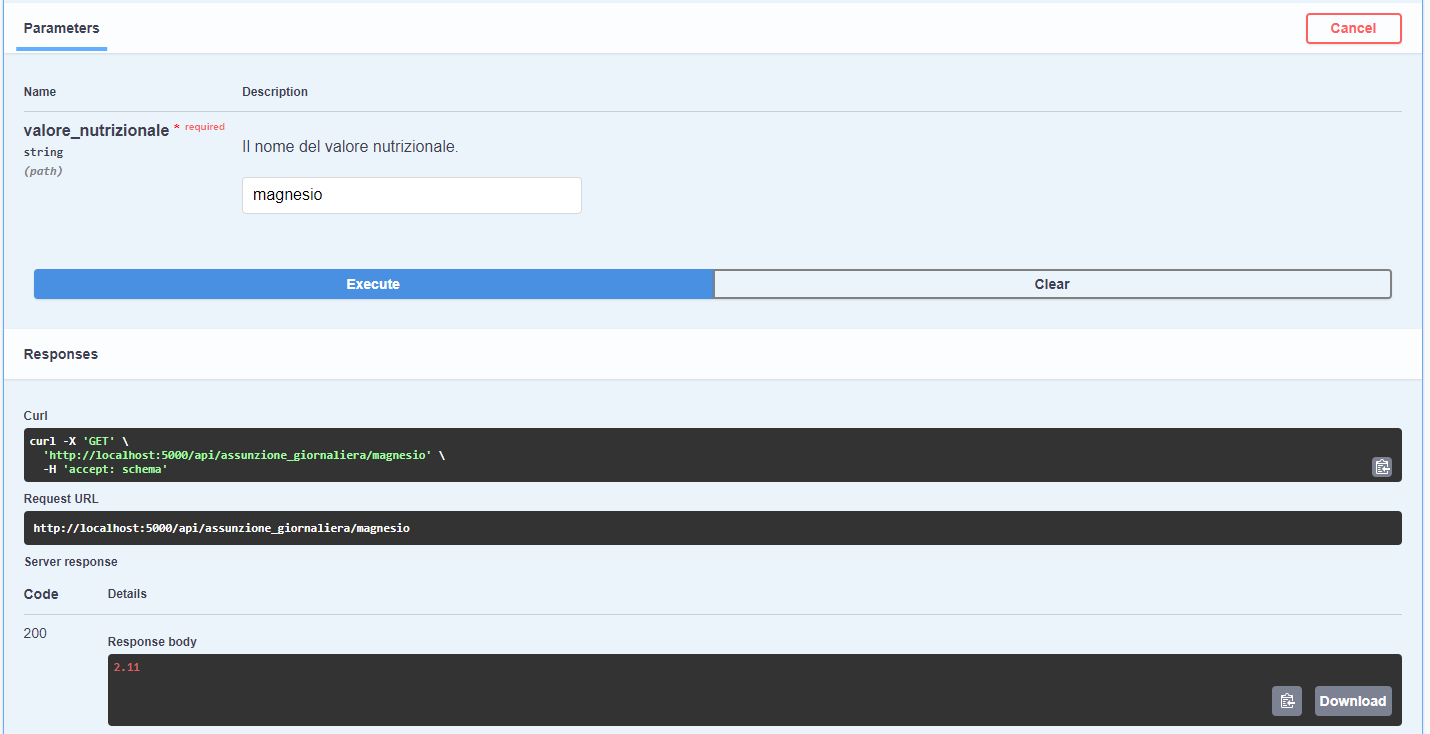
\includegraphics[scale=0.5]{risposta get assunzione_giornaliera.png}\\
   \\
   Si tiene a precisare che le API che richiedono un input da parte dell’utente, quindi tutte le POST e DELETE, e due API GET di utilità, non generano errori in caso di input errati. Quantità / Tempo / Data possono anche essere nulli, negativi o NaN e l’API semplicemente ritorna un codice di errore come risposta, come illustrato nella documentazione. Lo stesso vale per il database, se ci cerca di inserire una consumazione che non è presente, le due API che ne fanno uso riportano semplicemente l’errore 404. Ugualmente anche per JSON di input malformati o con valori non corretti, o per un tentativo di eliminazione di un’attività o una consumazione non presente nella cronologia.\\
   \section{FrontEnd Implementation}
   Il Front end fornisce le funzionalità di visualizzazione, inserimento e cancellazione dei dati nell’applicazione SmartFit. Permette di utilizzare tutte le API sviluppate, con le varie schede che fornisce. Siamo consapevoli che sia abbastanza grezzo, quasi inguardabile, ma non avevamo mai fatto nulla di simile e avevamo concentrato davvero tutte le nostre forze nello sviluppo delle API e back end nelle settimane antecedenti, trascurando l’aspetto grafico.\\
   La prima scheda dell’applicazione è la scheda di riepilogo giornaliero, che verrà poi anche chiamata “Home - Riepilogo giornaliero” durante la navigazione delle altre schede:\\
   \\
   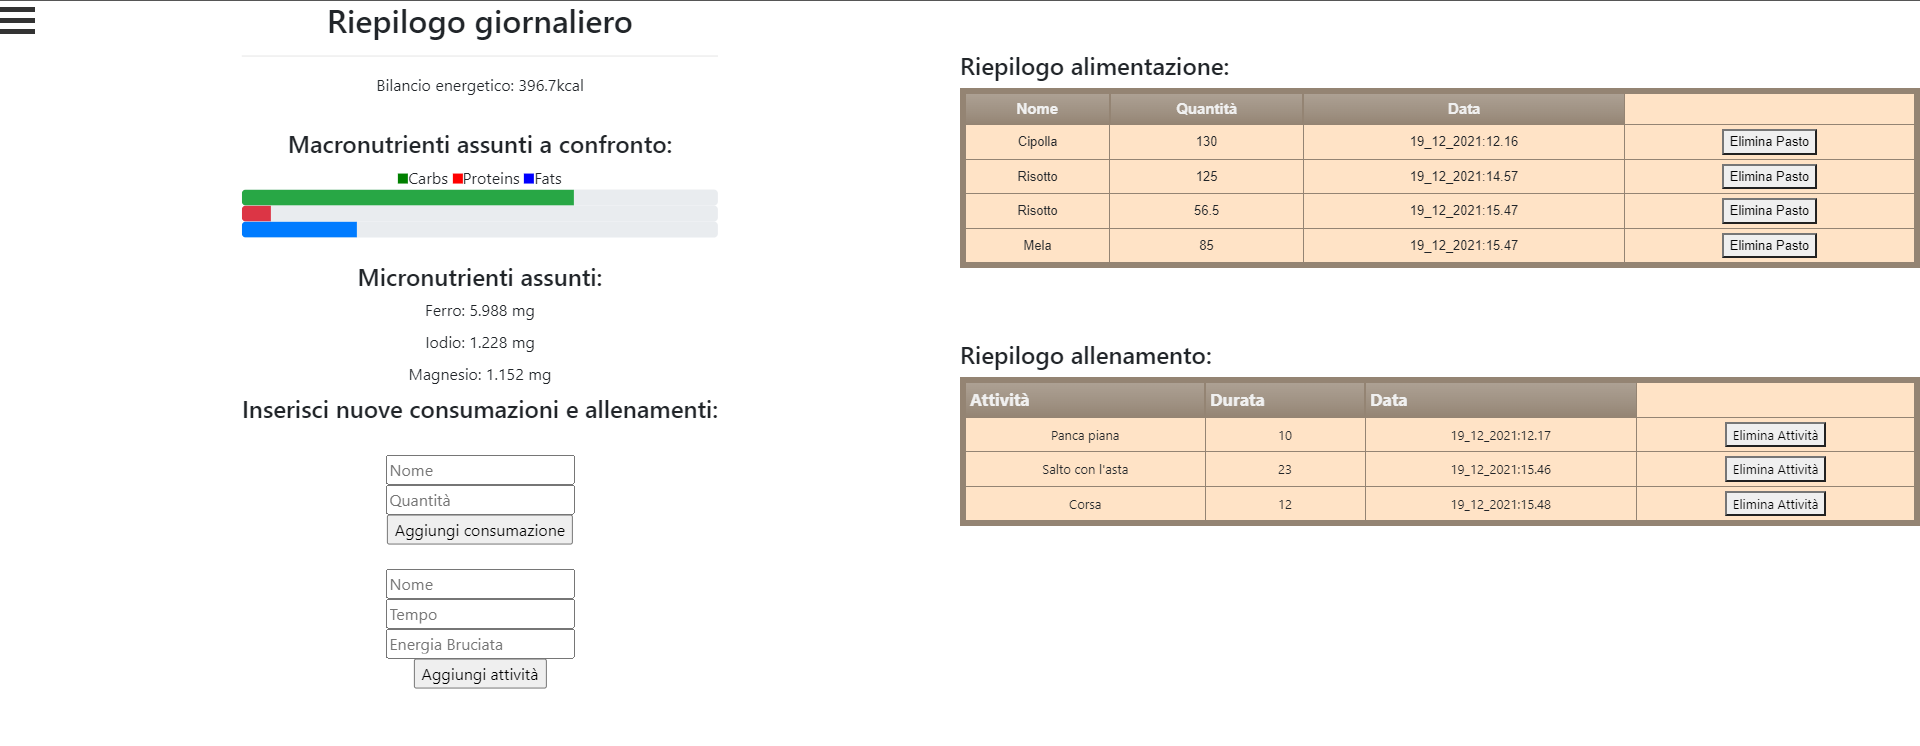
\includegraphics[scale=0.35]{riepilogo.png}\\
   Qui si possono vedere in azione la maggior parte delle API descritte precedentemente, e quindi anche la realizzazione di molte delle features elencate all’inizio del documento.
   Nella parte in alto a sinistra si possono trovare:
   \begin{itemize}
      \item Il bilancio energetico: differenza tra chilocalorie assunte e bruciate durante la giornata corrente, calcolato con l’ausilio delle due API GET di utilità nel back end, “calorie bruciate” e “calorie assunte".
      \item Le progress bar per confrontare l’assunzione giornaliera dei principali macronutrienti: il valore delle progress bar viene calcolato con un rapporto tra il risultato del valore ritornato dalla API GET “assunzione giornaliera” e il totale giornaliero assunto tra i vari macronutrienti.
      \item Le quantità di micronutrienti assunti: anche in questo caso viene utilizzata la API GET “assunzione giornaliera”.
   \end{itemize}
   Sempre sulla sinistra della scheda sono presenti i form per l’inserimento di nuove consumazioni e allenamenti. Queste utilizzano le API POST descritte in precedenza, ovvero “cronologia alimentazione” e "cronologia allenamento".\\

   A destra invece si possono trovare le tabelle con i riepiloghi giornalieri di alimentazione e allenamento. Le tabelle vengono create dinamicamente in base al JSON ritornato dalle due API GET di riepilogo, “riepilogo alimentazione” e “riepilogo allenamento”.
   Su ogni riga è presente il pulsante per eliminare la consumazione o l’attività presente su quella riga. Questi pulsanti poi chiamano le API DELETE “cronologia alimentazione” e “cronologia allenamento”.\\

   In alto a sinistra si trova il pulsante per aprire il menù che permette di raggiungere le altre schede:\\
   \begin{center}
      \includegraphics[scale=0.5]{menù.png}
   \end{center}
   Cliccando su “Cronologia pasti e allenamenti” ci si potrà recare alla scheda dove saranno presenti le tabelle con l’intera cronologia di alimentazione e allenamento. Le due tabelle sono create dinamicamente, utilizzando le API GET “cronologia allenamento” e “cronologia alimentazione”.\\
   \\
   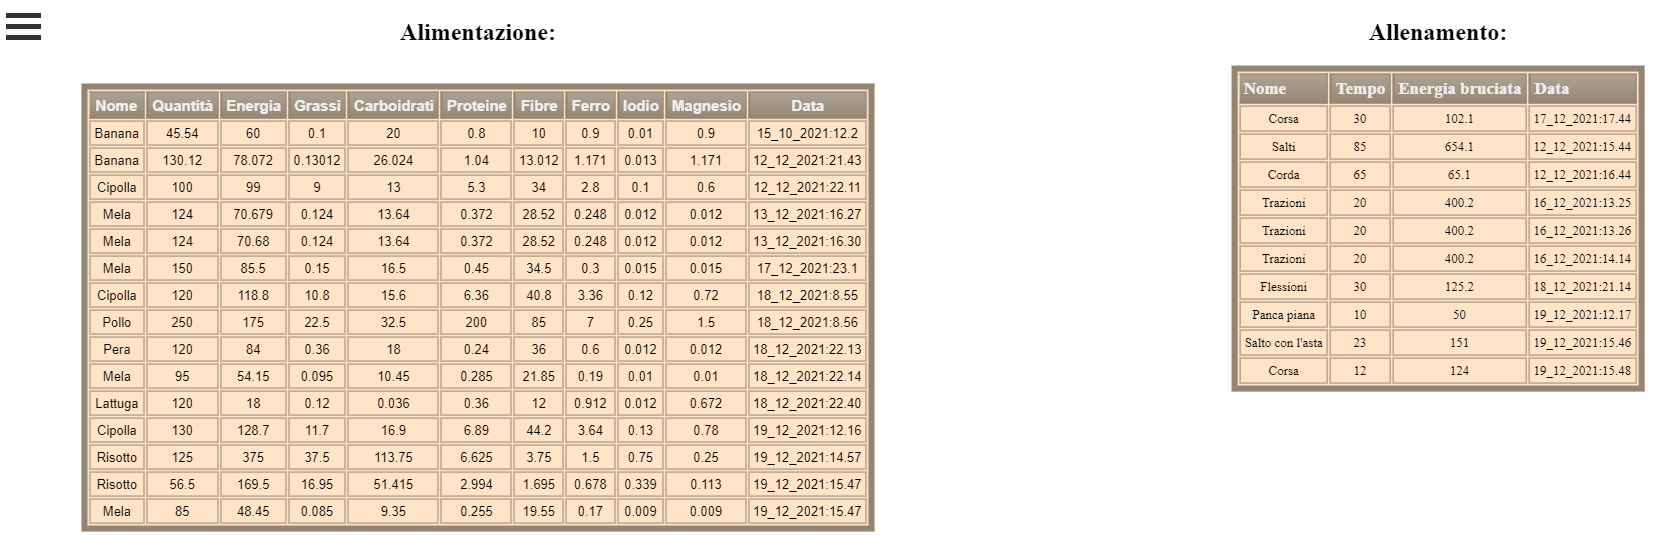
\includegraphics[scale=0.4]{cronologia.png}\\
   Sempre cliccando sull’icona a forma di hamburger ci si può spostare su altre schede come quella “Allenatore”:\\
   \\
   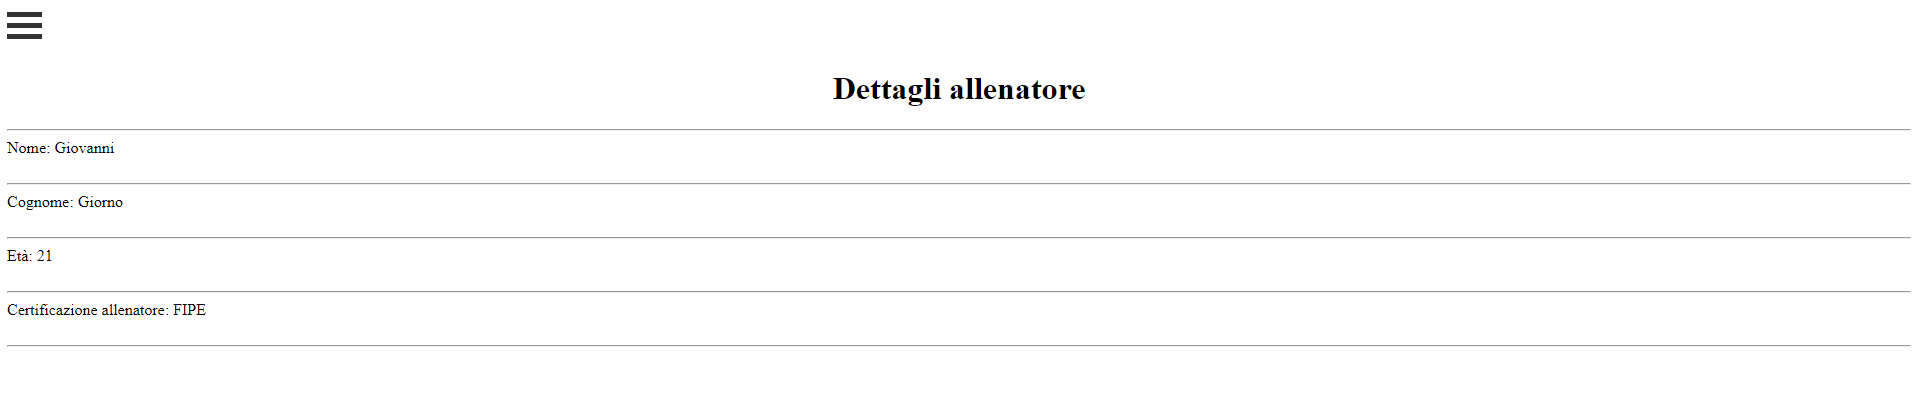
\includegraphics[scale=0.4]{allenatore.png}
   In questa schermata si possono vedere le informazioni sull’allenatore. Per recuperare tali informazioni si utilizza la API GET “dati allenatore".
   Infine, nella schermata “Le mie schede” si potranno vedere le due schede personalizzate:\\
   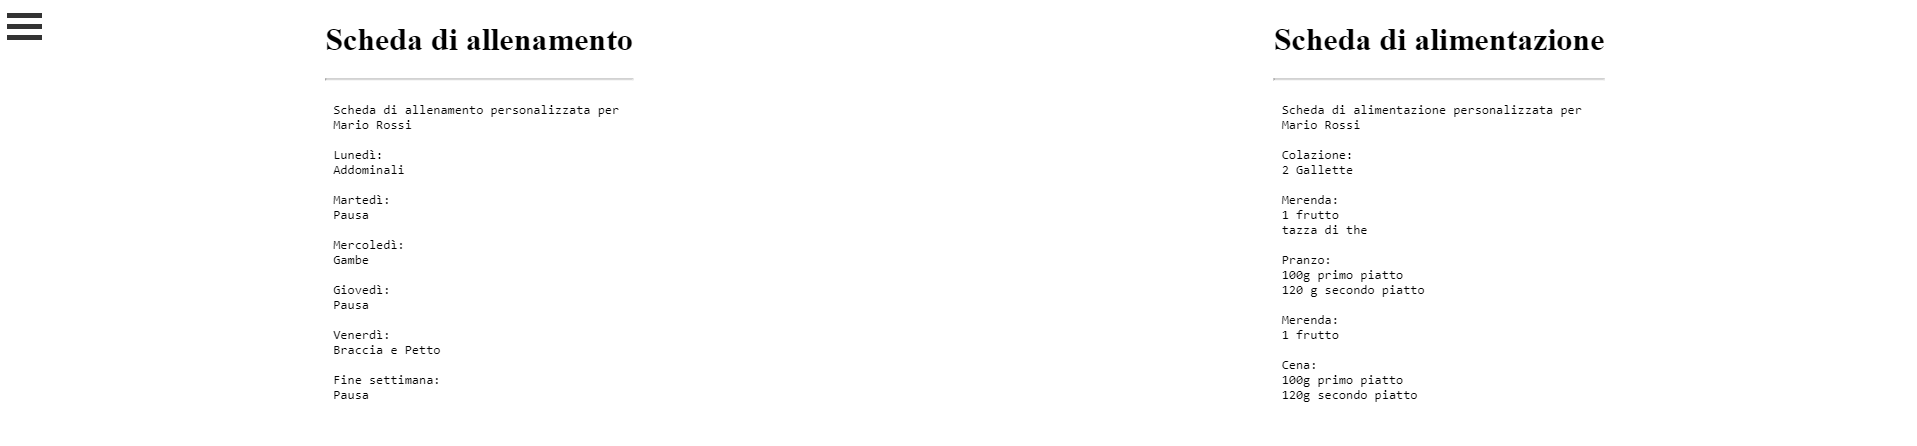
\includegraphics[scale=0.4]{schede personalizzate.png}
   \section{GitHub Repository Info}
   Il progetto SmartFit è disponibile al seguente link:\\

   \href{https://github.com/StellaDaniele/G12-software-engineering}{https://github.com/StellaDaniele/G12-software-engineering}\\

   Per poter eseguire il progetto è sufficiente recarsi all’interno della cartella api e poi eseguire il comando npm start. Il server, come verrà scritto in console, sarà in ascolto all’indirizzo \textit{localhost:5000/}
   \subsection{Stringa di connessione a MongoDB}
   Viene di seguito riportata la stringa di connessione al database MongoDB, che non volevamo inserire pubblica su GitHub e che comunque cambieremo appena l’esito verrà pubblicato.\\
   \\
   *****************************
   \section{API Testing}
   Per eseguire il testing abbiamo definito nel nostro progetto la cartella “test” nella cartella api. Al suo interno, è presente uno script index.js che va a definire alcuni test cases. Si è andato a verificare il corretto funzionamento di una API GET, di una API POST provando anche a inserire dati errati e che non rispettavano i requisiti per dimostrarne la robustezza, e infine di una DELETE, anch’essa viene provata con input errati per dimostrarne la robustezza.
   Per eseguire il test abbiamo modificato il file package.json inserendo la riga di codice per l’esecuzione dello script. Per avviare i test basta recarsi nella cartella \textbf{api} ed eseguire il comando \textit{npm test}. Si rammenta che dal momento che il server parte in ascolto, il testing non termina, per farlo terminare bisogna bloccare il server dal mettersi in ascolto dal file index.js nella cartella api.
   Questo è il risultato del testing:\\
   \begin{center}
      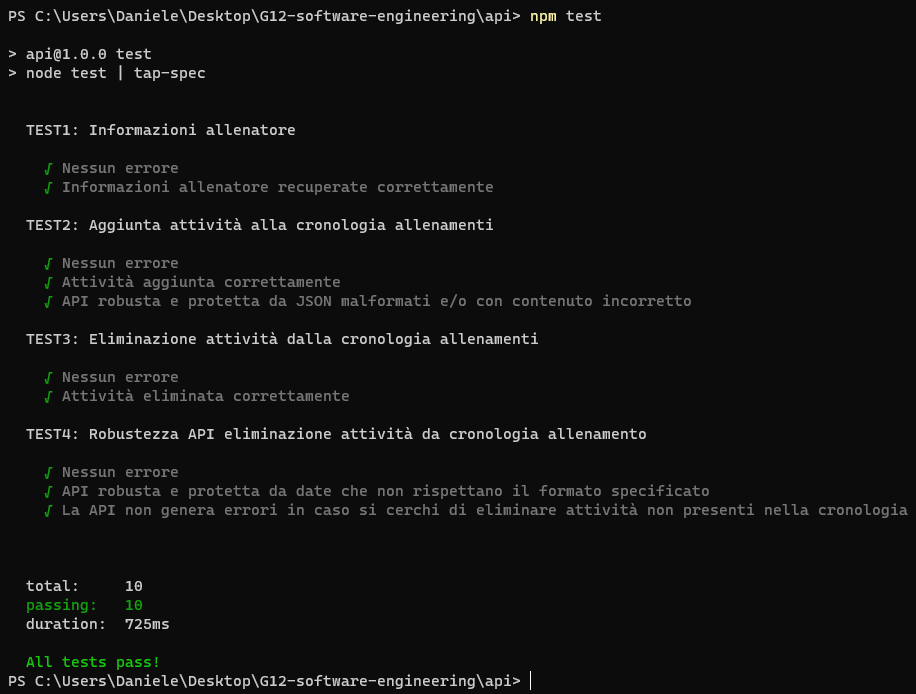
\includegraphics[scale=0.5]{testing API.png}
   \end{center}
\end{document}